\documentclass{article}
% translate with >> pdflatex -shell-escape <file>

% This file is an extract of the PGFPLOTS manual, copyright by Christian Feuersaenger.
% 
% Feel free to use it as long as you cite the pgfplots manual properly.
%
% See
%   http://pgfplots.sourceforge.net/pgfplots.pdf
% for the complete manual.
%
% Any required input files (for <plot table> or <plot file> or the table package) can be downloaded
% at
% http://www.ctan.org/tex-archive/graphics/pgf/contrib/pgfplots/doc/latex/
% and
% http://www.ctan.org/tex-archive/graphics/pgf/contrib/pgfplots/doc/latex/plotdata/

\usepackage{pgfplots}
\pgfplotsset{compat=newest}

\pagestyle{empty}

\usepgfplotslibrary{patchplots}

\begin{document}
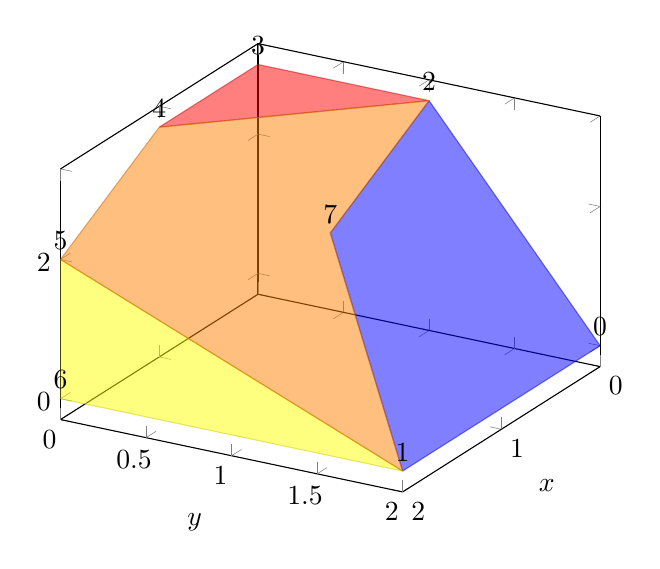
\begin{tikzpicture}
	\begin{axis}[view/h=120,xlabel=$x$,ylabel=$y$]
	\addplot3[
		opacity=0.5,
		table/row sep=\\,
		patch,
		patch type=polygon,
		vertex count=5,
		patch table with point meta={%
			% pt1 pt2 pt3 pt4 pt5 cdata
			0 1 7 2 2 0\\
			1 6 5 5 5 1\\
			1 5 4 2 7 2\\
			2 4 3 3 3 3\\
	}]
	table {
		x y z\\
		0 2 0\\%0
		2 2 0\\%1
		0 1 3\\%2
		0 0 3\\%3
		1 0 3\\%4
		2 0 2\\%5
		2 0 0\\%6
		1 1 2\\%7
	};
% replicate the vertex list to show \coordindex:
\addplot3[only marks,nodes near coords=\coordindex]
table[row sep=\\] {
0 2 0\\ 2 2 0\\ 0 1 3\\ 0 0 3\\ 
1 0 3\\ 2 0 2\\ 2 0 0\\ 1 1 2\\
};
	\end{axis}
\end{tikzpicture}
\end{document}
